\section{Linear Interpolation}
\label{example:LinearInterpolcation}

Linear interpolation is widely used to find the new value along the line determined by two data points. Figure \ref{fig:LinearInterpolation} shows how to find the linearly interpolated value from the two points $(x_0,y_0)$ and $(x_1,y_1)$ by the linear interpolant when $x_0 \le x \le x_1$

\begin{equation}
\label{eq:LinearInterpolation}
\begin{split}
L(x) &= y_0+\frac {y_1-y_0}{x_1-x_0} (x-x_0) \\
     &= \left(1-\frac{x-x_0}{x_1-x_0}\right)\cdot y_0 + \frac{x-x_0}{x_1-x_0}\cdot y_1 \\
	 &= (1-w) \cdot y_0 + w \cdot y_1
\end{split}
\end{equation}

where

$$
w = \frac{x-x_0}{x_1-x_0}
$$

Graphically,

\begin{figure}[h]
\centering
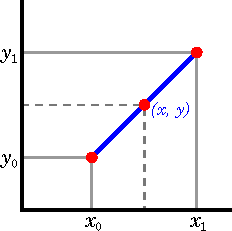
\includegraphics[width=8cm]{./figures/LinearInterpolation.pdf}
\caption{Linear interpolation}
\label{fig:LinearInterpolation}
\end{figure}


\subsection{Implementation}
In the implementation below, no linear extrapolation is performed for values outside the interval $[x_0, x_1]$. All the parameters of this function are simple numerical numbers. The first parameter is the $x$-coordinates of two data points and the second parameter is the $y$-coordinates of the two data points. The third parameter is the $x$-coordinate for the point to perform linear interpolation.

\begin{minted}[samepage,frame=single,framesep=10pt,xleftmargin=10pt,linenos]{q}
.math.lerp:{[x;y;z]
  if[2<>count x;'"First argument must be a two-element list"];
  if[x[0]>x 1;'"First argument must be in ascending order"];
  if[not z within x;:$[z<x 0;y 0;y 1]];
  w:%[z-x 0;x[1]-x 0];
  (1-w;w) wavg y
  };
\end{minted}

\subsection{Explanations}

\begin{itemize}
\item Line 2 checks the number of elements in the first parameter. It must have two elements. Otherwise an error is thrown.
\item Line 3 checks whether the second element is not smaller than the first element in the first parameter. Otherwise, an error is thrown.
\item Line 3 returns the $y$-coordinate value if $x$-coordinate is not within the interval defined by the two points.
\item Line 5 computes the weight for the value to interpolate
\item Line 6 calculates the weighted average
\end{itemize}


\subsection{Summary}

\begin{importantblock}
\textbf{Important Note}
\begin{itemize}
\item The argument \q{x} must be in ascending order in this implementation.
\end{itemize}
\end{importantblock}

\begin{noteblock}
\textbf{Knowledge Points}
\begin{itemize}
\item Functions \href{https://code.kx.com/q/ref/if/}{\q{if}}, \href{https://code.kx.com/q/ref/count/}{\q{count}}, \href{https://code.kx.com/q/ref/within/}{\q{within}} and \href{https://code.kx.com/q/ref/wavg/}{\q{wavg}} 
\item The if-else like conditional selection: \href{https://code.kx.com/q/ref/cond/}{\q{$}}
\item Error signalling: \href{https://code.kx.com/q/ref/signal/}{\q{'}}
\end{itemize}
\end{noteblock}

\clearpage
